% Chapter Template

\chapter{Ensayos y resultados} % Main chapter title

\label{Chapter4} % Change X to a consecutive number; for referencing this chapter elsewhere, use \ref{ChapterX}

%----------------------------------------------------------------------------------------
%	SECTION 1
%----------------------------------------------------------------------------------------
En este capítulo se describen los ensayos realizados y se presentan y comparan los resultados obtenidos.

\section{Banco de pruebas}
\label{sec:pruebasHW}

Para el desarrollo del presente proyecto se utilizaron 3 bancos de pruebas, con las siguientes especificaciones técnicas:

\begin{itemize}
\item Banco de pruebas \textit{Laptop} \textit{MacBook Pro} - \textit{hardware} disponible:
	\begin{itemize}
	\item \textbf{OS}: \textit{MacOS Sonoma} 14.
	\item \textbf{CPU}: Apple M1 Pro.
	\item \textbf{RAM}: 32 GB.
	\item \textbf{GPU}: No contiene.
	\end{itemize}
\item Banco de pruebas \textit{Laptop} \textit{ASUS TUF GAMING F15} - \textit{hardware} disponible:
	\begin{itemize}
	\item \textbf{OS}: \textit{Windows} 11.
	\item \textbf{CPU}: \textit{Intel(R) Core(TM)} i5-11260H.
	\item \textbf{RAM}: 16 GB.
	\item \textbf{GPU}: \textit{NVIDIA GeForce RTX} 3050.
	\end{itemize}
\item Banco de pruebas \textit{Google Colab Pro} - \textit{hardware} disponible:
	\begin{itemize}
	\item \textbf{OS}: desconocido.
	\item \textbf{CPU}: desconocido.
	\item \textbf{RAM}: 12,5 GB.
	\item \textbf{GPU}: T4.
	\end{itemize}
\end{itemize}

\section{Desempeño de modelos}
\label{sec:desempeñoMod}

Para medir el desempeño de los modelos de AI utilizados durante la ejecución de este proyecto, se decidió emplear la métrica \textit{mAP}. Esta métrica evalúa tanto la clasificación del objeto como la ubicación del \textit{bounding box} a través del \textit{Avarage Precision} (\textit{AP}) que se representa en la ecuación \ref{eq:AP}.

\begin{equation}
    \label{eq:AP}
    \text{AP} = \frac{1}{n} \sum_{k=1}^n \text{Precisión en } k \times \text{Rel}_{k}
\end{equation}

Siendo
\begin{itemize}
    \item \( n \) el número total de elementos recuperados.
    \item \(\text{Precision at } k\) la precisión en el \( k \)-ésimo punto de recuperación.
    \item \(\text{Rel}_{k}\) un indicador binario que denota si el elemento en el \( k \)-ésimo punto de recuperación es relevante (\( \text{Rel}_{k} = 1 \)) o no relevante (\( \text{Rel}_{k} = 0 \)).
\end{itemize}

Luego, al promediar los valores de \textit{AP} entre todas las clases, se obtiene respectivamente el \textit{mAP} y la ecuación quedaría como se muestra en \ref{eq:mAP}.

\begin{equation}
    \label{eq:mAP}
    \text{mAP} = \frac{1}{C} \sum_{c=1}^C \text{AP}_c
\end{equation}

Donde 
\begin{itemize}
	\item \( C \) es el número total de clases o consultas.
    \item \( AP \) es el Average Precision calculado para la clase o consulta.
\end{itemize}

\subsection{Desempeño del detector de regla}

El detector de la regla como se mencionó en el capítulo anterior,  tiene como modelo base un \textit{YOLOv8n} y cumple una función fundamental para la estimación de la longitud de la vareta. Por otro lado, el entrenamiento de este modelo se realizó con los siguientes hiperparámetros:

\begin{itemize}
	\item Epocas: 100.
    \item Tamaño de imagen de entrada: 640 x 640.
    \item \textit{Batch}: 16.
    \item \textit{Learning rate}: 0.01.
\end{itemize}

Los resultados obtenidos para la detección de este elemento contra el conjunto de datos de prueba se observan en la tabla \ref{tab:resultadosRegla}.

\begin{table}[h]
	\centering
	\caption{Métricas de detección para el detector de regla.}
	\begin{tabular}{c c c c c c c}    
		\toprule
		\textbf{Clase}&\textbf{Imágenes}&\textbf{Objetos encontrados}&\textbf{Precision} &\textbf{Recall}&\textbf{mAP 50}&\textbf{mAP 50-95}\\
		\midrule
		Regla & 13 & 13 & 0.996 & 1.0 & 0.995 & 0.995\\		
		\bottomrule
		\hline
	\end{tabular}
	\label{tab:resultadosRegla}
\end{table}

Los resultados fueron muy buenos en general. El modelo puede detectar la regla sin dificultad en el 99\% de los casos.

\subsection{Desempeño del detector de vareta}

El detector de vareta destinado para el módulo de estimación de longitud, tiene como modelo base un \textit{YOLOv8n} entrenado bajo los siguientes hiperparámetros:

\begin{itemize}
	\item Epocas: 100.
    \item Tamaño de imagen de entrada: 640 x 640.
    \item \textit{Batch}: 16.
    \item \textit{Learning rate}: 0.01.
\end{itemize}

Para este modelo se hicieron dos prubas, una sin aumento de datos y otra con aumento. El aumento de datos aplicado se describe en la sección \ref{aumentoDatos}.

Los resultados obtenidos contra el conjunto de datos de pruebas para el modelo sin aumento de datos se muestran en la tabla \ref{tab:resultadosVareta}.

\begin{table}[h]
	\centering
	\caption{Métricas de detección para el detector de varetas sin aumento de datos.}
	\begin{tabular}{c c c c c c c}    
		\toprule
		\textbf{Clase}&\textbf{Imágenes}&\textbf{Objetos encontrados}&\textbf{Precision} &\textbf{Recall}&\textbf{mAP 50}&\textbf{mAP 50-95}\\
		\midrule
		Vareta & 10 & 40 & 1.0 & 0.923 & 0.983 & 0.574\\		
		\bottomrule
		\hline
	\end{tabular}
	\label{tab:resultadosVareta}
\end{table}

Como se puede observar, el modelo sin aumento de datos, consigue detectar un total de 40 varetas en 10 imágenes, donde todas las detecciones fueron correctas. Por otro lado, el modelo logra una precisión promedio de detección del 98.3\% cuando se requiere un nivel de confianza igual al 50\%, pero el \textit{mAP} 50-95, indica que en los casos donde el nivel de confianza esta entre el 50\% y 95\%, la precisión promedio, es de un 57.4\%. Por este motivo, se decidió aplicar aumento de datos.

Los resultados con aumento de datos se pueden observar en la tabla \ref{tab:resultadosVaretaConAug}.

\begin{table}[h]
	\centering
	\caption{Métricas de detección para el detector de varetas con aumento de datos.}
	\begin{tabular}{c c c c c c c}    
		\toprule
		\textbf{Clase}&\textbf{Imágenes}&\textbf{Objetos encontrados}&\textbf{Precision} &\textbf{Recall}&\textbf{mAP 50}&\textbf{mAP 50-95}\\
		\midrule
		Vareta & 10 & 40 & 0.974 & 0.975 & 0.976 & 0.702\\		
		\bottomrule
		\hline
	\end{tabular}
	\label{tab:resultadosVaretaConAug}
\end{table}

Luego de aplicar aumento de datos, se observa que, el modelo mejoró la cantidad de veces donde detecta de forma precisa a la clase vareta en un 5.2\% con respecto al modelo sin aumento de datos. Por otro lado, también se incrementó la precisión promedio al 70.2\% cuando se tiene un umbral de confianza que va entre 50\% y 95\%.

Con esto se destaca que, el aumento de datos mejoró el rendimiento del modelo de forma considerable.

\subsection{Desempeño del detector de estados fenológicos}

La detección de estados fenológicos, como se mencionó en el capítulo anterior, fue probada con dos modelos de IA que se ajustan para este caso de uso. Por un lado, se probó con un detector de dos etapas como es \textit{Faster R-CNN} y por otro lado con un detector de una etapa como \textit{YOLOv8}. Ambos casos, se probaron con y sin el uso de aumento de datos. Los resultados fueron los siguientes:

\subsubsection{\textit{Faster R-CNN} sin aumento de datos}

El entrenamiento del modelo se hizo bajo los siguientes hiperparámentros:

\begin{itemize}
	\item Epocas: 100.
    \item Tamaño de imagen de entrada: 640 x 640.
    \item \textit{Batch}: 4.
    \item \textit{Learning rate}: 0.001.
    \item \textit{Momentum}: 0.9.
    \item \textit{Weight decay}: 0.0005.
    \item \textit{Optimizer}: \textit{Stochastic gradient descent}.
\end{itemize}

Los resultados de detección contra el conjunto de prueba se muestra en la tabla \ref{tab:resultadosFasterSinAug}.

\begin{table}[h]
	\centering
	\caption{Métricas de detección para \textit{Faster R-CNN} sin aumento de datos.}
	\begin{tabular}{c c c c c c c}    
		\toprule
		\textbf{Clase}&\textbf{Imágenes}&\textbf{mAP}&\textbf{mAP 50}&\textbf{mAP > 50}\\
		\midrule
		Todas & 14 & 0.3492 & 0.5970 & 0.3605\\
		Flor abierta & 14 & 0.4313 & - & - \\
		Flor cerrada & 14 & 0.1525 & - & - \\
		Flor sin pétalos & 14 & 0.3735 & - & - \\
		Incierto & 14 & 0.0942 & - & - \\
		Vareta & 14 & 0.6947 & - & - \\		
		\bottomrule
		\hline
	\end{tabular}
	\label{tab:resultadosFasterSinAug}
\end{table}

La precisión promedio de detección entre todas las clases es de un 34.9\%, lo que significa que, el modelo tiene una precisión del 34.9\% al detectar las diferentes clases en el conjunto de datos. Además, El modelo logra una precisión de detección del 59.7\% cuando se considera un umbral de confianza igual al 50\% y para detecciones con un nivel de confianza mayor al 50\% se tiene una precisión del 36.1\%.

Por otro lado, al evaluar la precisión promedio de detección por clase, se observa que la categoría \textit{vareta}, es la clase a la que el modelo detecta con mejor precisión promedio con 69.5\%, seguida por \textit{flor abierta} con 43.13\% y por \textit{flor sin pétalos} con 37.35\%. Además, se muestra que el modelo detecta con dificultad las categorías \textit{flor cerrada} con un \textit{mAP} de 12.25\% e \textit{incierto} con 9.42\%.

Este bajo porcentaje de \textit{mAP} para la clase \textit{flor cerrada} con respecto a las otras categorías presentes, se puede deber al desbalance de datos observado en la sección \ref{desbalanceAfterLabeled} y al rendimiento del modelo al intentar detectar objetos pequeños en la imagen. Adicionalmente, para la categoría \textit{incierto} no se cuenta con una cantidad de muestras significativas y consistente a través del conjunto de datos, lo que explica la baja precisión promedio obtenida para esta clase.

Para mejorar estos resultados se implementó el aumento de datos mencionado en la sección \ref{aumentoDatos}.

\subsubsection{\textit{Faster R-CNN} con aumento de datos}

El rendimiento del modelo basado en la métrica \textit{mAP}, se puede observar en la tabla \ref{tab:resultadosFasterConAug}. 

\begin{table}[h]
	\centering
	\caption{Métricas de detección para \textit{Faster R-CNN} con aumento de datos.}
	\begin{tabular}{c c c c c c c}    
		\toprule
		\textbf{Clase}&\textbf{Imágenes}&\textbf{mAP}&\textbf{mAP 50}&\textbf{mAP > 50}\\
		\midrule
		Todas & 14 & 0.3733 & 0.6328 & 0.3793\\
		Flor abierta & 14 & 0.5143 & - & - \\
		Flor cerrada & 14 & 0.2049 & - & - \\
		Flor sin pétalos & 14 & 0.3290 & - & - \\
		Incierto & 14 & 0.0887 & - & - \\
		Vareta & 14 & 0.7294 & - & - \\		
		\bottomrule
		\hline
	\end{tabular}
	\label{tab:resultadosFasterConAug}
\end{table}
\newpage
Como se puede observar, se logra mejorar la precisión promedio de detección para las clases \textit{flor abierta}, \textit{flor cerrada} y \textit{vareta}. Con esto, la métrica \textit{mAP} medida entre todas las clases mejora a 37.33\%, adicionalmente también aumenta a 63.26\% cuando se fija un umbral de confianza de detección igual al 50\% y a un 37.93\% cuando el nivel de confianza en la detección es superior al 50\%.

Se puede concluir que el modelo \textit{Faster R-CNN} con y sin aumento de datos es bueno para detectar la vareta y las flores en estado abierto. Este comportamiento se puede deber al tamaño de estos objetos en la imagen en comparación con el resto de las categorías que se busca en la detección. Además, la clase \textit{flor abierta} es la clase más predominante en todas las imágenes según el estudio de los datos realizado en la sección \ref{desbalanceAfterLabeled}, lo que permite que el modelo pueda aprender y reconocer con mayor precisión sus características debido a la abundancia de ejemplos representativos durante el entrenamiento.

\subsubsection{\textit{YOLOv8n} sin aumento de datos}

El resultado obtenido con \textit{YOLOv8n} sin aumento de datos, con 14 imágenes del conjunto de pruebas y bajo los siguientes parámetros de entrenamiento:

\begin{itemize}
	\item Epocas: 100.
    \item Tamaño de imagen de entrada: 640 x 640.
    \item \textit{Batch}: 16.
    \item \textit{Learning rate}: 0.01.
\end{itemize}

Se puede observar en la tabla \ref{tab:resultadosYoloSinAug}.

\begin{table}[h]
	\centering
	\caption{Métricas de detección para \textit{YOLOv8n} sin aumento de datos.}
	\begin{tabular}{c c c c c c c}    
		\toprule
		\textbf{Clase}&\textbf{Imágenes}&\textbf{mAP 50}&\textbf{mAP > 50}\\
		\midrule
		Todas & 14 & 0.645 & 0.418\\
		Flor abierta & 14 & 0.905 & 0.611 \\
		Flor cerrada & 14 & 0.614 & 0.251 \\
		Flor sin pétalos & 14 & 0.588 & 0.363 \\
		Incierto & 14 & 0.122 & 0.065 \\
		Vareta & 14 & 0.994 & 0.802 \\		
		\bottomrule
		\hline
	\end{tabular}
	\label{tab:resultadosYoloSinAug}
\end{table}

Se puede observar que \textit{YOLOv8n} tiene una precisión promedio, entre todas las clases, cuando se fija un umbral del 50\% de 64.5\%, que supera al \textit{mAP} 50 obtenido con el modelo \textit{Faster R-CNN} con y sin aumento de datos.

Las clases que este modelo detecta con más precisión son: vareta, flor abierta y flor cerrada. La diferencia y mejora contra \textit{Faster R-CNN} se puede observar también al comparar la métrica \textit{mAP} obtenida para todas las clases donde este modelo se desempeño mejor. Como ejemplo se tiene la clase \textit{vareta} donde se obtuvo un 69.5\% y, con \textit{YOLOv8n}, esta misma clase que también fue la mejor para este modelo tuvo 99.4\% que representa una mejora del 29.9\%.

Por otro lado la clase \textit{vareta}, en general, ambos modelos la logran detectar con alta precisión y esto se puede deber al tamaño de este objeto en la imagen. Además, es seguida por la clase \textit{flor abierta} que, como se mencionó anteriormente, contiene una cantidad de muestras representativas que ayudan al modelo a reconocer los patrones de esta clase. Por último, se destaca la categoría \textit{incierto}, que tanto este modelo como \textit{Faster R-CNN} no logran reconocer durante la detección en su totalidad.

La matriz de confusión normalizada mostrada en la figura \ref{fig:cfmatriznorm}, indica que muchas de las veces que se tiene la clase \textit{incierto}, el modelo la predice como \textit{flor abierta}. Lo que demuestra que el modelo durante el entrenamiento no logró aprender correctamente los patrones que identifican dicha clase.

\begin{figure}[ht]
	\centering
	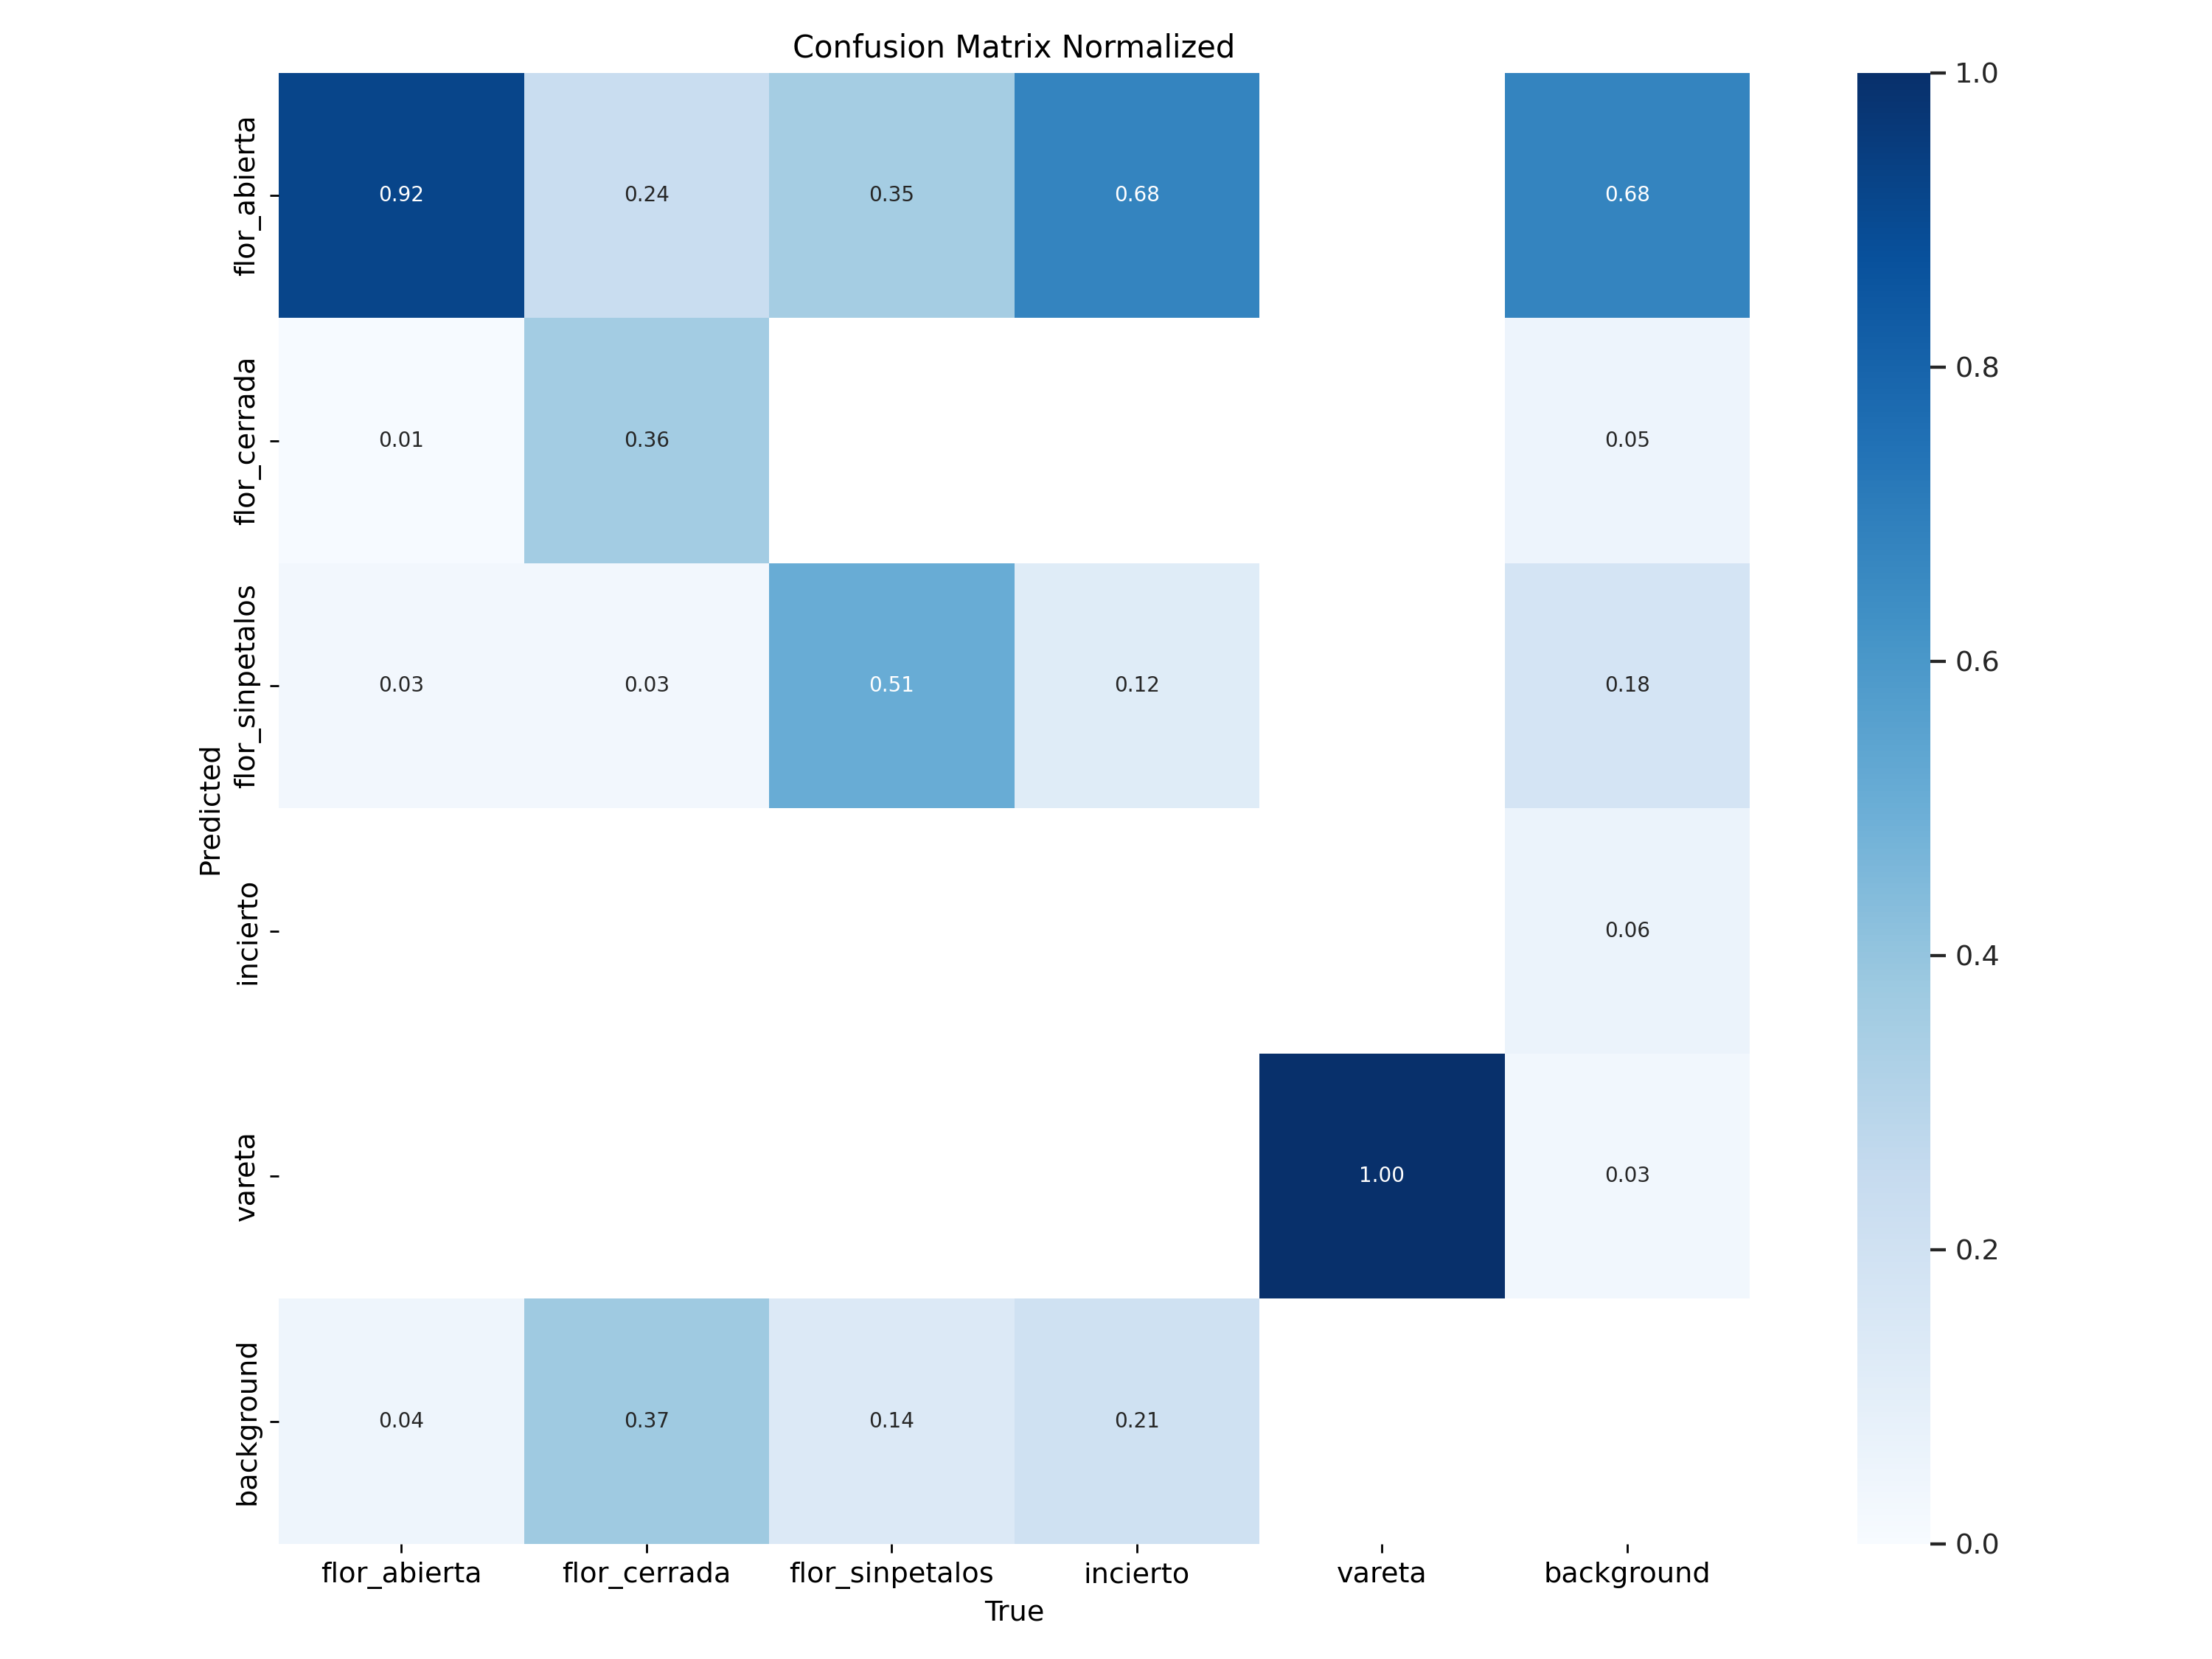
\includegraphics[scale=0.52]{./Figures/CFMatrixnorm.png}
	\caption{Matriz de confusión normalizada de \textit{YOLOv8n} para el conjunto de prueba.}
	\label{fig:cfmatriznorm}
\end{figure}

\subsubsection{\textit{YOLOv8n} con aumento de datos}

Para mejorar los resultados de \textit{YOLOv8n} se implementó el aumento de datos descrito en la sección \ref{aumentoDatos}. Los resultados obtenidos contra el conjunto de imágenes de prueba, se observa en la tabla \ref{tab:resultadosYoloConAug}.

\begin{table}[h]
	\centering
	\caption{Métricas de detección para \textit{YOLOv8n} con aumento de datos.}
	\begin{tabular}{c c c c c c c}    
		\toprule
		\textbf{Clase}&\textbf{Imágenes}&\textbf{mAP 50}&\textbf{mAP > 50}\\
		\midrule
		Todas & 14 & 0.655 & 0.423\\
		Flor abierta & 14 & 0.893 & 0.611 \\
		Flor cerrada & 14 & 0.673 & 0.266 \\
		Flor sin pétalos & 14 & 0.603 & 0.373 \\
		Incierto & 14 & 0.111 & 0.065 \\
		Vareta & 14 & 0.995 & 0.802 \\		
		\bottomrule
		\hline
	\end{tabular}
	\label{tab:resultadosYoloConAug}
\end{table}

La precisión promedio para un umbral de confianza igual al 50\% mejora para la clase \textit{flor cerrada} en un 5.9\% , para la clase \textit{flor sin pétalos} en un 1.5\%. Mientras que se tiene una perdida para la clase flor abierta del 1.2\%. Quedando el \textit{mAP} 50 entre todas las clases con un aumento del 1\%.

Se observa que el entrenamiento del modelo con aumento de datos ayudó a mejorar el reconocimiento de las clases más difíciles de detectar como son \textit{flor cerrada} y \textit{flor sin pétalos}. Además, mantiene el buen rendimiento para las clases \textit{flor abierta} y \textit{vareta}.

Al comparar todos los experimentos realizados para la detección de los estados fenológicos de las flores de duraznero, el modelo con mejor rendimiento basado en la métrica \textit{mAP} para dicha tarea es \textit{YOLOv8n} con aumento de datos. Por este motivo, se seleccionó este modelo para desempeñar dicha tarea.

Por último, se aplicó \textit{Eigen-CAM} \cite{ARTICLE:17} para crear mapas de calor que permitan explicar los resultados obtenidos por el modelo. Este mapa de calor se implementó en la capa convolucional \textit{C2f}. En la figura \ref{fig:EigenCam}, se observa un ejemplo de los mapas de calor generados por \textit{Eigen-CAM} en una foto perteneciente al conjunto de pruebas utilizando \textit{YOLOv8n} con aumento de datos.

\begin{figure}[ht]
	\centering
	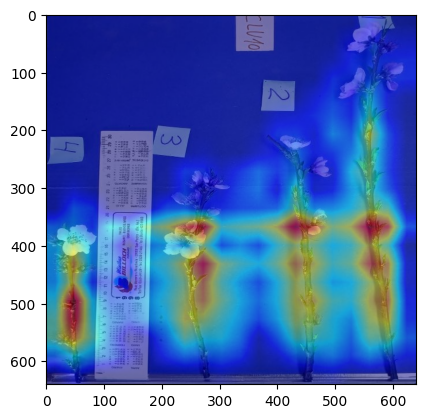
\includegraphics[scale=0.55]{./Figures/EigenCamEj.png}
	\caption{Mapa de calor con \textit{Eigen-CAM} en la capa \textit{C2f} del modelo \textit{YOLOv8n}.}
	\label{fig:EigenCam}
\end{figure}
\newpage

Se observa que los mapas de activación están enfocados en las varetas para la capa convolucional seleccionada, lo que sugiere que el modelo pone mayor atención en este objeto al realizar la detección.   


\section{Desempeño de módulos}
\label{sec:desempeñoModulos}